\ylDisplay{Uppuv klots} % Ülesande nimi
{Tundmatu autor} % Autor
{lõppvoor} % Voor
{2012} % Aasta
{P 10} % Ülesande nr.
{3} % Raskustase
{
% Teema: Mehaanika

\ifStatement
Vees ujub vahtrapuust kuup servapikkusega $a = 10$ cm tihedusega $\rho_{vaher} = 700$ $kg/m^3$ . Kuubi sees on silindriline õõnsus läbimõõduga $b = 4,5$ cm (vt. joonist). Õõnsus on alt suletud õhukese korgiga. 
a) Arvutage, kas kuup upub, kui õõnsus täita liivaga? Liiva tihedus on $\rho_{liiv} = 2700$ $kg/m_3$ ja vee tihedus on $\rho_{vesi} = 1000$ $kg/m^3$. 
b) Kui korgile mõjuv summaarne jõud on suurem kui $1,8$ N, läheb kork katki. 
Mis on maksimaalne liiva kõrgus, mida saab õõnsusesse valada?
\begin{center}
	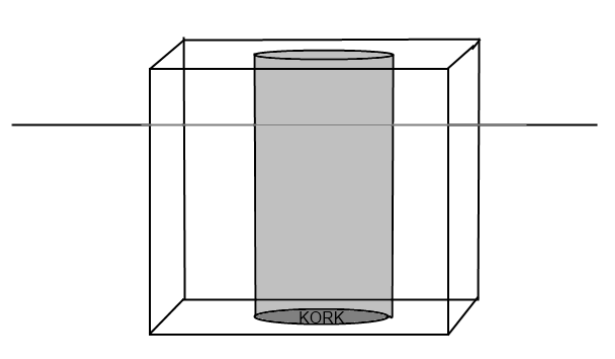
\includegraphics[width=0.5\linewidth]{2012-v3p-10-yl.PNG}
\end{center}
\fi

\ifHint
Korgile mõjub liiva raskusjõud ning altpoolt surub seda vesi. Kork kannatab nende jõudude vahet.
\fi

\ifSolution
$a)$ Leiame maksimaalse raskusjõu ja üleslükkejõu ning vaatame, kas üleslükkejõud on väiksem kui raskusjõud.
\begin{center}
$F_r = F_{klots} + F_{liiv} = (\rho_{vaher}(a^3 - \pi b^2 \frac{a}{4}) + \rho_{liiv} \pi b^2 \frac{a}{4})g = 9,975$ N
\end{center}
\begin{center}
$F_y = \rho_{vesi} ga^3 = 9,8$ $N$
\end{center}
Seega klots on võimalik ära uputada.
\newline
$b)$ Korgile mõjub liiva raskusjõud ning altpoolt surub seda vesi. Kork kannatab nende jõudude vahet. $S = \pi b^2/4$ - augu põhja pindala, $h$ liivasamba kõrgus, $A$ - klotsi vee alla ulatuva osa kõrgus.
\begin{center}
$1, 8 N = \rho_{liiv}Shg - \rho_{vesi}g AS$
\end{center}
Teise seose saame panna kirja klotsi ujumise tingimustest.
\begin{center}
$F_r = F_y$
\end{center}
\begin{center}
$(\rho_{vaher}(a^3 - Sa) + \rho_{liiv} Sh)g = \rho_{vesi}ga^2 A$
\end{center}
Lahendades need võrrandid, saame, et $A = 0.092m = 9,2$ cm ning $h = 0,0768$ m = $7,68$ cm. Ehk kork eelamdub enne kuubiku uppumist ja seega ei saa kuubikut sellel viisil uputada.
\fi
}